As we described earlier, in \namd{} GPU design all nonbonded work 
is offloaded to GPU since its computation is most intensive.
In code shown in ~\ref{gpu-cpu-assignment}, it is implemented by assigning computes to GPU so long as 
it has the types of Nonbonded*, which include NonbondedPair and
NonbondedSelf.  

%\begin{lstlisting}[float,frame=single,caption={Compute Assignment},label=gpu-cpu-assignment]
\begin{lstlisting}[frame=single,caption={Compute Assignment},label=gpu-cpu-assignment]
switch ( type of compute )    
{
    case computeNonbondedSelfType:
            register_cuda_compute_self(i,map->computeData[i].pids[0].pid);
            break;
    case computeNonbondedPairType:
            register_cuda_compute_pair(i,pid2,trans2);
            break
   ........................
   other types:
            create computes on CPU
            break;
}

\end{lstlisting}

\textbf{Motivation} : While this is a straightforward way to balance load between CPU and GPU, 
it may have significant performance problem depending on the configuration
of GPU and CPU.

Figure~\ref{figs:gpu-ppn1} and ~\ref{figs:gpu-ppn15} show the timeline of 
running $92,224$ atom Apoa1 using 1 GPU and 1 CPU core, 1GPU and 15 CPU cores.
Each main line represents execution on one CPU core. Different colors stand for 
different function execution. The red activity is for integration while the purple
is all bonded work on CPU. The white color stands for idle time. The green bars on top of the main bars 
show the execution of GPU. In Figure~\ref{figs:gpu-ppn1}, the total time range 
is around $117 ms$, which is the time for one simulation step. We can see that
GPU only takes a small portion of total time, which is around $19 ms$.
In this case, it is correct that we should offload as much nonboned work as possible
to GPU since CPU execution is relatively slow. 

However, in Figure~\ref{figs:gpu-ppn15} when we increase the number of CPU cores, 
the work on CPU side is parallelized and time is reduced to $12 ms $ while the GPU exection
still takes $19 ms$. As a result, on CPU side, there is a big portion of idle time.    

\begin{figure}[h]
\centering
\subfigure[1CPU core + 1 GPU] {\label{figs:gpu-ppn1}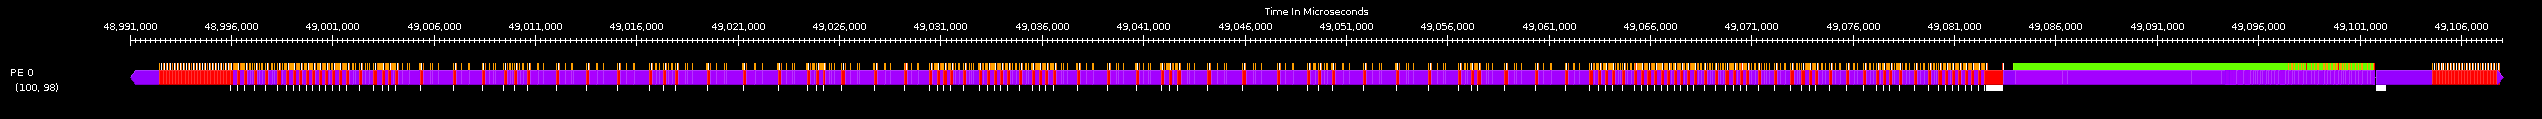
\includegraphics[width=5.8in]{figs/gpu-ppn1-timeline-117ms.png}}
\subfigure[15 CPU cores + 1 GPU] {\label{figs:gpu-ppn15}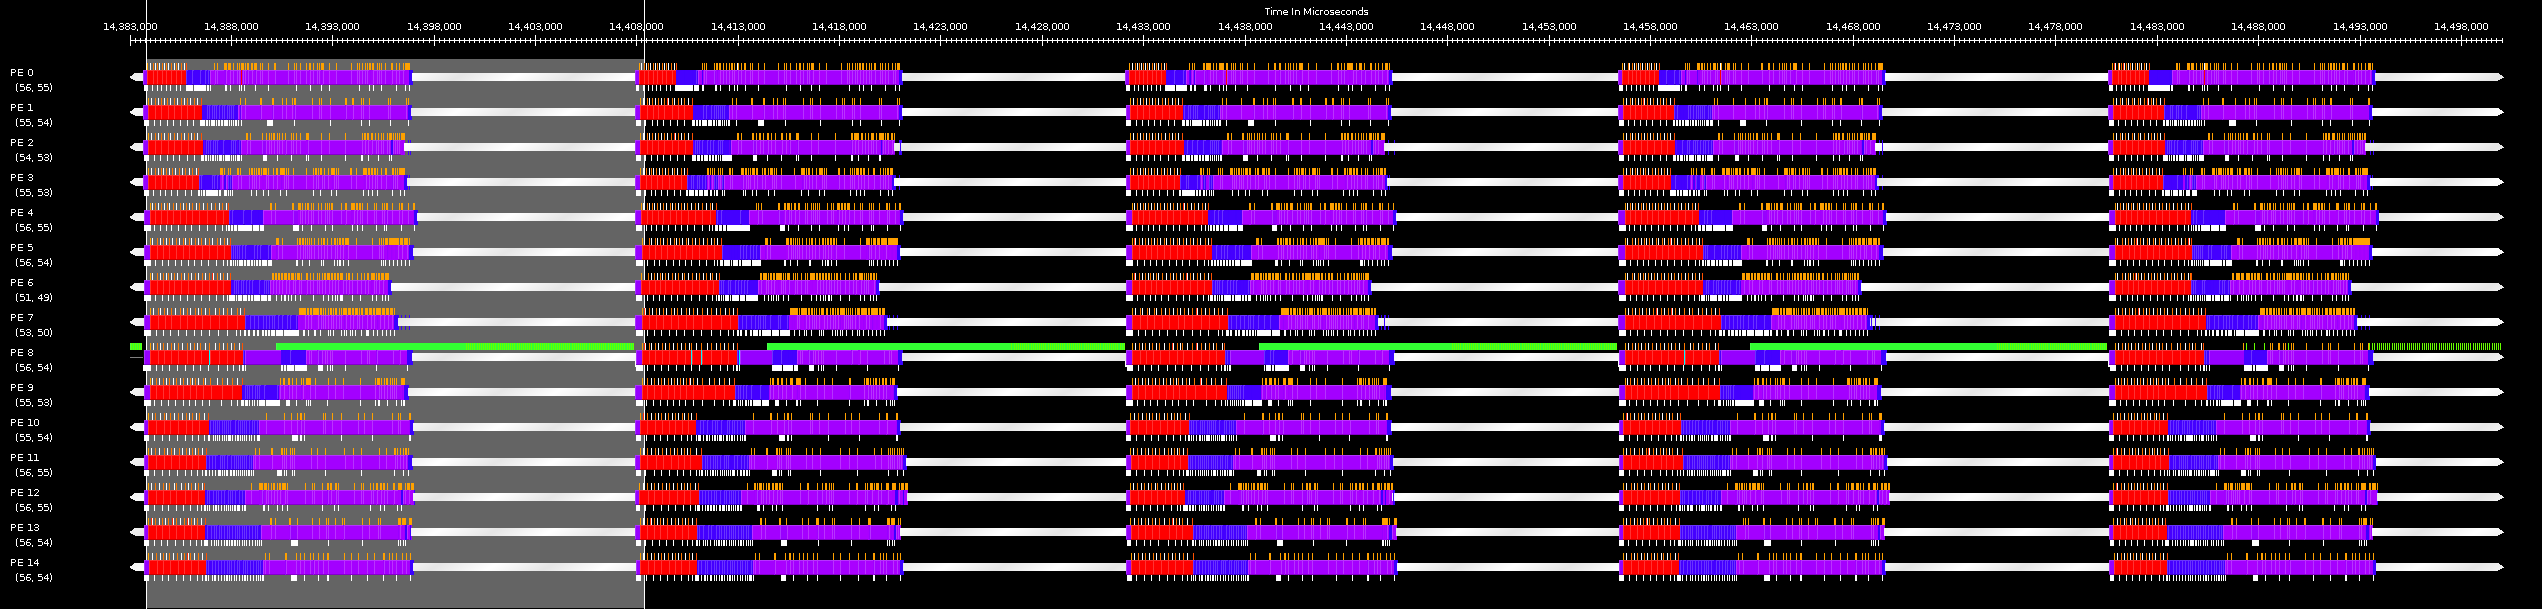
\includegraphics[width=5.8in]{figs/gpu-ppn15-timeline-117-25ms.png}}
\caption{Timeline of running Apoa1 with 1 GPU and different number of CPU cores}
\label{figs:cpu-gpu}
\end{figure}


